\documentclass[11pt]{article}
\usepackage[margin=1in]{geometry}
\usepackage{mathpazo}
\usepackage{amsmath,amssymb}
\usepackage{microtype}
\usepackage{booktabs}
\usepackage{graphicx}
\usepackage[dvipsnames]{xcolor}
\usepackage{tikz}
\usetikzlibrary{positioning,arrows.meta,calc,fit,backgrounds}
\usepackage[most]{tcolorbox}
\usepackage{enumitem}
\usepackage{listings}
\usepackage[font=small,labelfont=bf]{caption}
\usepackage{hyperref}
\hypersetup{colorlinks=true,linkcolor=MidnightBlue,citecolor=MidnightBlue,urlcolor=MidnightBlue}
\usepackage{cleveref}
\urlstyle{tt}
\def\UrlBreaks{\do\_\do/\do.}
\newcommand{\file}[1]{\nolinkurl{#1}}
\newcommand{\code}[1]{\texttt{#1}}
\newcommand{\mhh}{m_{hh}}
\newcommand{\bw}{\boldsymbol{\omega}}
\newcommand{\bp}{\boldsymbol{p}}
\newcommand{\bx}{\boldsymbol{x}}
\newcommand{\data}{\mathcal{D}}

\definecolor{trainable}{HTML}{1B6CA8}
\definecolor{physics}{HTML}{2E933C}
\definecolor{datac}{HTML}{7B4EA3}
\definecolor{warn}{HTML}{C0392B}

\newtcolorbox{keyidea}[1][]{enhanced,breakable,colback=physics!6,colframe=physics!70!black,
  fonttitle=\bfseries,title={#1},boxrule=0.6pt,arc=2pt,left=6pt,right=6pt}
\newtcolorbox{aside}[1][]{enhanced,breakable,colback=trainable!5,colframe=trainable!70!black,
  fonttitle=\bfseries,title={#1},boxrule=0.6pt,arc=2pt,left=6pt,right=6pt}
\newtcolorbox{assume}[1][]{enhanced,breakable,colback=datac!5,colframe=datac!70!black,
  fonttitle=\bfseries,title={#1},boxrule=0.6pt,arc=2pt,left=6pt,right=6pt}
\newtcolorbox{watch}[1][]{enhanced,breakable,colback=warn!5,colframe=warn!70!black,
  fonttitle=\bfseries,title={#1},boxrule=0.6pt,arc=2pt,left=6pt,right=6pt}
\setlist{itemsep=2pt,topsep=3pt}
\setlength{\emergencystretch}{3em}

\lstset{language=Python, basicstyle=\ttfamily\small, columns=fullflexible,
  keepspaces=true, commentstyle=\color{physics!70!black}\itshape,
  keywordstyle=\color{trainable!90!black}\bfseries, stringstyle=\color{datac},
  showstringspaces=false, frame=single, rulecolor=\color{gray!40},
  backgroundcolor=\color{gray!3}, xleftmargin=4pt, xrightmargin=4pt,
  aboveskip=6pt, belowskip=6pt}

\title{\textbf{The POWHEG spectra are scaled event counts}\\[4pt]
\large Recovering the counts and the scale factor of every spectrum}
\date{October 31, 2026}
\begin{document}
\maketitle

\begin{keyidea}[Summary]
\begin{enumerate}
  \item Every spectrum, training and test, is \emph{exactly} $t_k = q_s n_k$ with one scale
    factor $q_s$ per spectrum and integer counts $n_k$; the largest deviation of any
    $t_k/q_s$ from an integer is $4\times10^{-4}$, the precision of the single-precision
    numbers in the files.
  \item The noise variance is therefore $q_s t_k$ exactly; the global
    $N_\text{eff} = 38{,}024$ is no longer needed. It overstated the variance by 2.7\% for
    a typical spectrum, and understated it by a factor 2.5 for the two short runs in the
    training file (IDs 1814 and 4284, about 15,000--16,000 events).
  \item Every run generated 40,000 events (confirmed by the colleague who produced them);
    the events missing from the binned range fall below 255 or above 1455~GeV. The two
    short spectra (IDs 1814 and 4284) do not fit: they would need about 24,000 events
    outside the range, while their first and last bins suggest a few hundred; their
    normalisation is nevertheless right, so they are most likely runs of about 16,000
    events.
  \item There is no sign of common random numbers between spectra.
  \item New module \file{dihiggs/counts.py}; it processes the training file in 2 seconds.
\end{enumerate}
\end{keyidea}

\section{Method}

If all events of a run carry the weight $q_s$, the cross sections of the bins of
spectrum $s$ are integer multiples of $q_s$, and $q_s$ is their greatest common divisor.
Let $t_\text{min}$ be the smallest non-zero value. If that bin holds $c$ events, every
ratio $c\,t_k/t_\text{min}$ is an integer. We try $c = 1, 2, \ldots$ and keep the first $c$
for which all ratios are within 0.01 of an integer; then $n_k = \mathrm{round}(c\,t_k /
t_\text{min})$ and $q_s = \sum_k t_k / \sum_k n_k$. The first $c$ gives the largest $q_s$;
a smaller one ($q_s/2$, say) would be selected instead only if every count of the spectrum
were even, which for about 80 bins does not happen. The count $c$ of the smallest bin ranges
from 1 (in 15\% of the spectra) to 177, with a median of 14. A spurious, smaller $c$ would
require about 80 ratios to fall within 0.01 of an integer by chance, a probability of
about $0.02^{80}$.

\section{Results}

\begin{figure}[h]
\centering
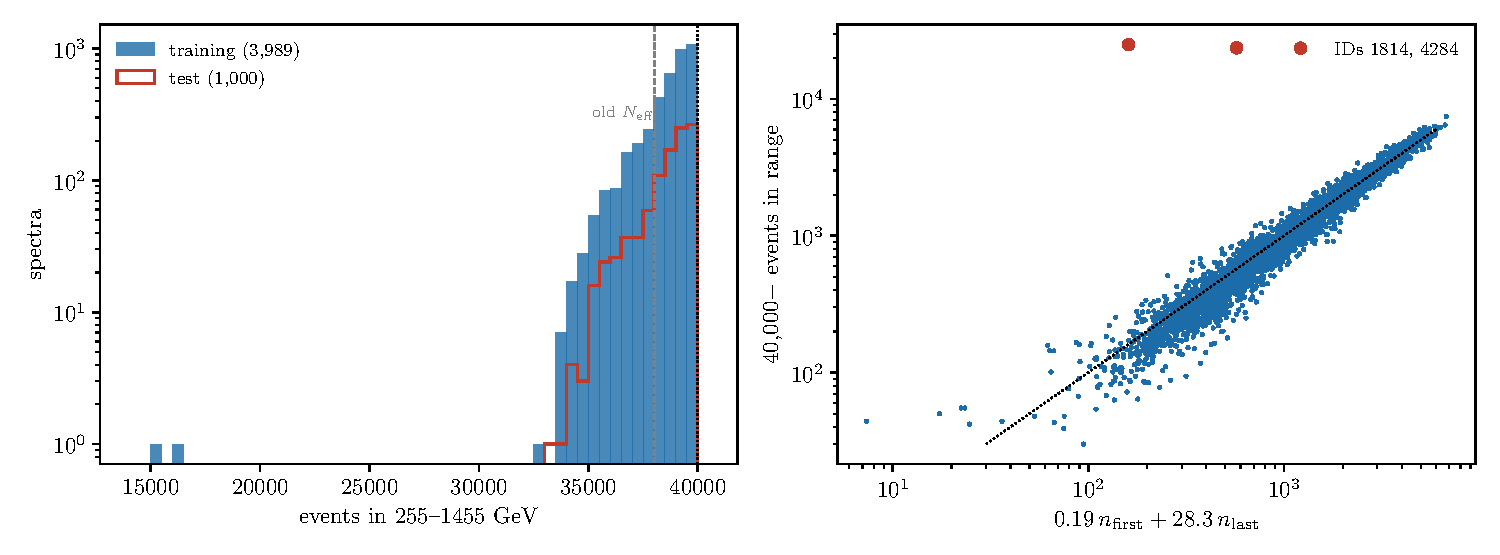
\includegraphics[width=\textwidth]{fig_counts.pdf}
\caption{Left: the number of events inside the binned range, for the training (filled)
and test (line) spectra; the dotted line marks 40,000, the dashed line the old
$N_\text{eff}$. Right: the number of events missing from 40,000 against a simple proxy for
the number expected outside the range (a fit of $a\,n_\text{first} + b\,n_\text{last}$,
the counts in the first and last bins); correlation 0.986. The two short runs (red) are
far off the line.}
\label{fig:counts}
\end{figure}

\begin{itemize}
  \item \textbf{All spectra are exact multiples.} Training: 3,989 of 3,989; test: 1,000
    of 1,000. Largest deviation $4.0\times10^{-4}$ of a count, for counts up to about
    8,000, i.e.\ a relative precision of $5\times10^{-8}$: single-precision rounding.
  \item \textbf{Events in range} (\cref{fig:counts}, left): median 39,043 (training) and
    39,041 (test); 5\% of the training spectra have fewer than 36,061. The largest is
    39,970. Two training spectra, IDs 1814 and 4284, have only 15,031 and 16,310
    events. If every run generated 40,000 events, about 24,000 of theirs are unaccounted for.
    Their normalisation is right, however: their total cross sections agree with the
    ensemble's prediction at their HEFT points to 0.5\% and 0.2\%. So these runs most likely
    produced only about 16,000 events and were normalised to the events they had. They are
    valid histograms with their own $q_s$, which the method finds automatically; only their
    noise is larger. % TODO (HBP): confirm with the colleague.
  \item \textbf{40,000 generated events.} If every complete run generated 40,000 events,
    the deficit $40{,}000 - N_\text{in}$ is the number of events below 255 or above
    1455~GeV. A crude proxy built from the first and last bins tracks it with correlation
    0.986 (\cref{fig:counts}, right), with no spectrum above 40,000, as expected: every run
    generated 40,000 events (confirmed by the colleague who produced the samples).
  \item \textbf{Empty bins.} 1,814 bins with no events were dropped from the training file
    (the test file keeps them as zeros). \code{add\_empty\_bins} restores them.
\end{itemize}

\section{Independence}

\paragraph{Within a spectrum.} Counts with a fixed total are multinomial, not independent (every run generated 40,000 events):
$\mathrm{Cov}(n_i, n_j) = -N p_i p_j$, a correlation of about $-\sqrt{p_ip_j}$, at most a
few per cent here; the counts in range are multinomial together with the out-of-range
events. A multinomial likelihood equals a
product of independent Poisson likelihoods with the normalisation of the spectrum left
free; treating the bins as independent Poisson therefore overstates only the information
on each spectrum's total, by one count's worth among about 80 bins. We neglect it. The
scale factor $q_s = \sigma_\text{tot}/N_\text{gen}$ also carries POWHEG's integration error
on $\sigma_\text{tot}$, common to all bins of a spectrum; its size is not known to us.
% TODO (HBP): the POWHEG integration error on sigma_tot, if available.

\paragraph{Between spectra.} Independence requires a different random seed for every
run. Using the difference of each bin from the mean of its two neighbours, a model-free
estimate of its fluctuation, the correlation between pairs of test spectra over the 58
bins above 555~GeV averages $0.0006$; there is no common fluctuation.

\section{Consequences}

\begin{table}[h]
\centering
\small
\begin{tabular}{lccccc}
\toprule
fine-tuned bootstrap ensemble & \multicolumn{3}{c}{s.d.\ of pull} & \multicolumn{2}{c}{$\langle\chi^2\rangle$ per bin} \\
 & all & 255--555 GeV & $>555$ GeV & 255--555 GeV & $>555$ GeV \\
\midrule
old variance, $t_k\sigma_\text{tot}/N_\text{eff}$ & 1.069 & 1.145 & 1.042 & 1.62 & 1.10 \\
exact variance, $q_s t_k$ & 1.077 & 1.153 & 1.050 & 1.65 & 1.12 \\
\bottomrule
\end{tabular}
\caption{The test-spectrum results of the appendix with the exact variances. The ratio
of old to exact variance on the test spectra has median 1.027 and ranges from 0.88 to
1.05.}
\end{table}

\begin{itemize}
  \item The appendix numbers move by about 1\%; the model-error coefficient will rise
    slightly. The noise model was, if anything, too generous, so the model error is not an
    artefact of an underestimated noise.
  \item For the Laplace approximation and any Poisson likelihood, the weight of a bin is
    $1/(q_s f_k)$, with $f_k$ the prediction (\code{poisson\_variance(df, prediction=f)}),
    which also covers empty bins and bins with a single event.
  \item The training noise variance $(t_k + u_k)u_k$ of the fine-tune becomes
    $q_s\,(t_k + q_s)$, or $q_s f_k$; the fine-tune itself need not be redone for the
    paper, since its result is validated on the test spectra.
\end{itemize}

\section{Code}

\begin{lstlisting}
from dihiggs import counts
out, summary = counts.recover_counts(df)        # adds 'count' and 'quantum'
full = counts.add_empty_bins(out)               # 80 bins per spectrum
var = counts.poisson_variance(full)             # q * t
var_f = counts.poisson_variance(full, prediction=f)   # q * f
n, q, dev = counts.recover_counts_wide(F)       # test file: one row per spectrum
\end{lstlisting}

\end{document}
